\chapter{Background}

This chapter introduces relevant background information on
best practice guidelines (\BPG{}) and guidelines-based clinical decision support
systems (\CDSS{}).
In section \ref{sec:bpg-background}, we utilize a real-world \BPG{}
to explain the motivation behind codifying treatment
in the form of clinical guidelines. We also briefly discuss
common characteristics of such guidelines that enable medical knowledge
to be represented efficiently and accurately.

\BPGs{} are usually published by hospitals,
research institutions and medical associations with the aim to improve quality of care by
\begin{enumerate*}[label=(\alph*)]
  \item reducing medical errors due to preventable causes,
  \item standardizing knowledge from latest evidence-based research, and,
  \item enabling access to aforementioned knowledge at medical establishments
  that lack resources to conduct research.
\end{enumerate*}

While in theory, following \BPGs{} should improve clinical outcomes,
their effectiveness in practice is dictated by whether healthcare practitioners
follow them or not. In section \ref{sec:cdss-background}, we present
challenges that practitioners encounter in following \BPGs{}. We then argue
that non-conformance results in worse patient outcomes.
Next, we show how computerized systems that utilize data from available
heterogeneous sources such as electronic health records and sensors for
patient parameters can improve patient outcomes by addressing challenges
to following \BPGs{} encountered by practitioners.

\section{Clinical Best Practice Guidelines}\label{sec:bpg-background}

Clinical best practice guidelines are evidence-based statements
published by hospital and medical associations that codify recommended
interventions for various clinical scenarios
\cite{field1990clinical}. High quality guidelines are routinely updated to account for
 results from clinical trials and advances in medicine, and make the latest
 diagnosis and treatment information accessible to providers \cite{SteinbergNAP11}.

\begin{figure}[t]
  \centering
  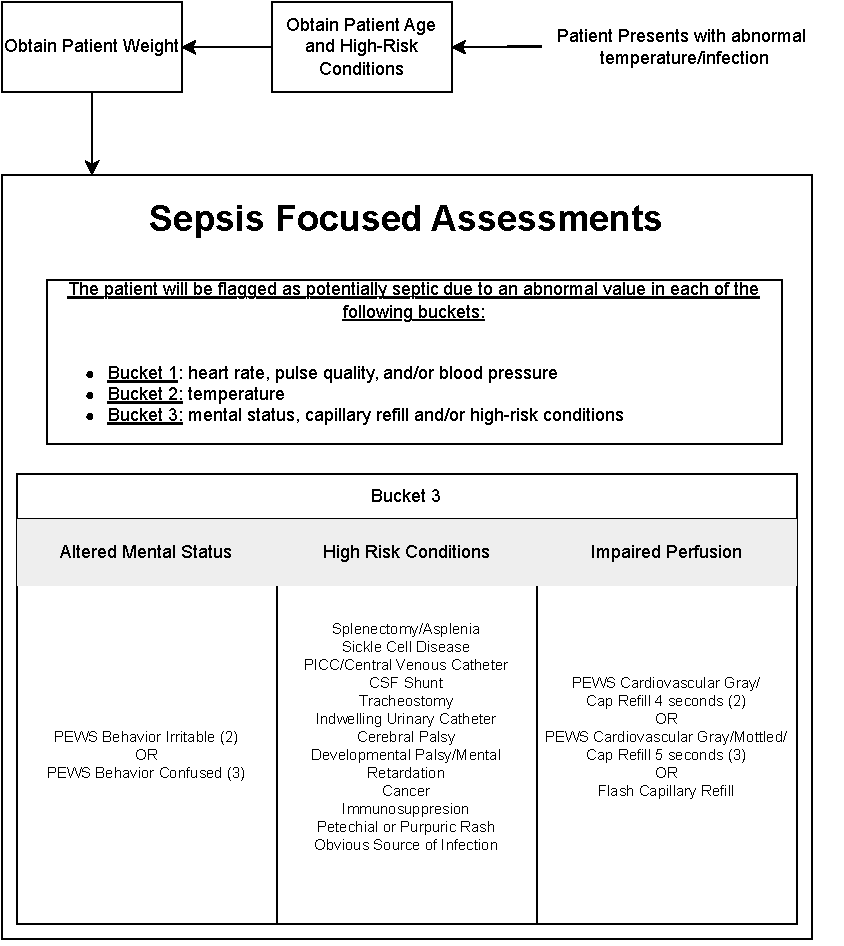
\includegraphics[width=0.5\textwidth]{sepsis-screening-osf}
  %\includegraphics[width=0.5\textwidth]{screening-vitals}
  \caption{Pediatric sepsis screening \BPG{}}\label{fig:sepsis-screening}
\end{figure}

To illustrate characteristics of \BPGs{}, we briefly go over a \BPG{}
for managing sepsis in pediatric cases used at OSF St. Francis Medical Center
in Peoria, Illinois -- a major pediatric hospital in the United States. Note
that for brevity, we refer to said hospital simply as OSF in the remainder of
this section.
Sepsis is life-threatening condition caused by the body's extreme response to
an infection \cite{RhodesICM17}, and is
a major cause of morbidity and mortality in children \cite{Eisenberg2021JP}.
Adverse outcomes can, however, be mitigated through timely
identification and prompt treatment with antibiotics and
intravenous (IV) fluids \cite{Weiss2014CCM,Evans2018JAMA}.
\BPGs{} for screening and management of sepsis in pediatric Emergency
Departments (EDs) have shown effectiveness in screening and management of sepsis \cite{Eisenberg2021JP},
leading to their adoption in many pediatric EDs \cite{Balamuth2017EM,Sepanski2014FP}.

In \figurename{} \ref{fig:sepsis-screening}, we present a simplified version of
the screening section of OSF's sepsis mangement guideline.
In essence, when a patient arrives at the
\ED{} with a fever or an infection, the \HCP{} is supposed to obtain
\begin{enumerate*}[label=(\alph*)]
  \item the patient's age,
  \item any conditions, such as cancer, immunosuppresssion, etc,
    that increase likelihood of sepsis, and
  \item the patient's vital signs, such as heart rate, systolic blood
    pressure, respiratory rate, etc.
\end{enumerate*}

This information is then used to check for abnormalities
in clusters of linked information, called \say{buckets}. For instance, if
the patient's heart rate is abnormal, then \say{bucket 1} is said to
have an abnormal value.
Checking for such abnormalities often involves the use of tables, such as
\tablename{} \ref{table:vital-signs} that contains normal ranges indexed by
\emph{age}.
%\footnote{For brevity, we omit some age ranges and vital signs from table
%\ref{table:vital-signs}}.
If the patient has at least one abnormal value in every \say{bucket},
then he/she is flagged as potentially septic.

The \BPG{}-recommended treatment for
sepsis involves multiple concurrent workflows, such as
screening for septic shock, fluid resuscitation, and administering antibiotics.
In \figurename{} \ref{fig:fluid-therapy}, we provide
a version of the fluid resuscitation guideline used
at OSF. Briefly, if the patient is flagged as potentially septic, the guideline suggests
\begin{enumerate*}[label=(\roman*)]
  \item obtaining any fluid-overload risks,
  \item administering normal saline (typically over a period of 15 minutes),
    where the dosage is dictated by risks determined in previous step,
  \item assessing signs of fluid-overload,
  \item evaluating patient responsiveness to normal saline upon completion of
    the administering process, and,
  \item determining whether another fluid bolus should be administered based on
    information from previous steps.
\end{enumerate*}
\begin{figure}[b]
  \centering
  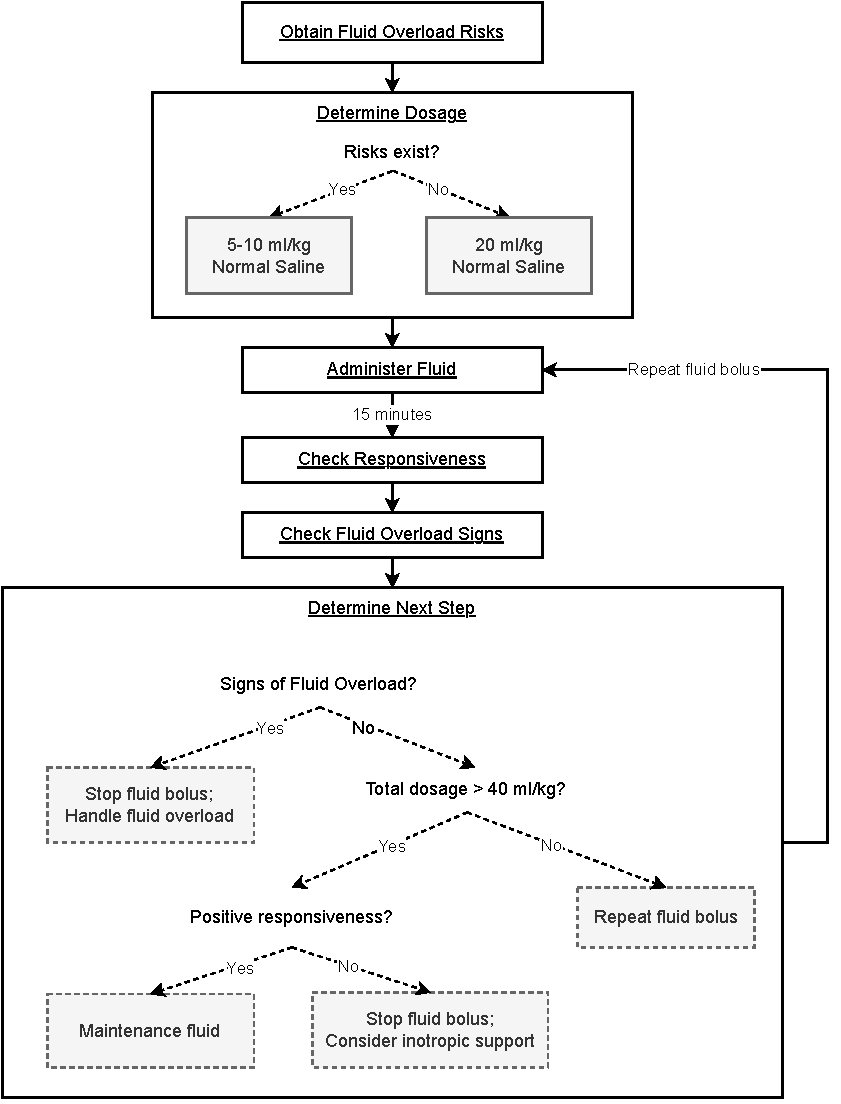
\includegraphics[scale=0.5]{FluidWorkflow-fmcad.pdf}
  \caption{Fluid Resuscitation Guideline}\label{fig:fluid-therapy}
\end{figure}

  \begin{table}
    \centering
    \begin{tabular}{ | c || c | c | c | }
      \hline
      \textbf{Age}            & \textbf{Heart Rate}   & \textbf{Systolic BP} & \textbf{Temp}  \\
      \hline
      $0d - 1m$               & $>205$                & $<60$                & $<36 \text{ or } >38$ \\
      \hline
      $\geq 1m - 3m$          & $>205$                & $<70$                & $<36 \text{ or } >38$ \\
      \hline
      $\geq 3m - 1y$          & $>190$                & $<70$                & $<36 \text{ or } >38.5$ \\
      \hline
      $\dots$                 & $\dots$               & $\dots$              & $\dots$ \\
      \hline
      $\geq 13y$              & $>100$                & $<90$                & $<36 \text{ or } >38.5$ \\
      \hline
    \end{tabular}
    \caption{Vital Signs Chart}\label{table:vital-signs}
  \end{table}

This real-world \BPG{} exhibits characteristics common
across many \BPGs{}. Specifically \BPGs{} typically:
\begin{itemize}
  \item Involve \stress{concurrent} workflows, such as administering drugs,
    monitoring vitals, performing treatment, etc. There may also be
    inter-workflow interactions. For instance, a diagnosis of sepsis during the
    screening may require modifications to an ongoing course antibitiotics.
  \item Often specified in a \stress{flowchart-like}
    notation. See \cite{AHAFlowcharts} and \cite{CancerCareFlowcharts} for other flowchart-based \BPGs{} for management of \emph{cardiac arrest}, and
    screening, risk-reduction, treatment and survivorship in
    cancer care respectively.
  \item Require communication between \stress{heterogeneous agents} such as
     monitors and Electronic Health Records (EHRs).
  \item Often use \stress{tables} indexed by parameters such as age, weight,
    etc to present normal/abnormal ranges for measurements, or recommended dosages for drugs.
\end{itemize}

Note that the aforementioned characteristics are \emph{not} specific
to one guideline. According to a review paper on \CIGs{} \cite{ClerqAIM03},
such \DSLs{} should additionally
\begin{enumerate*}[label=(\alph*)]
  \item be formally defined, i.e, have a formal syntax and semantics, and
  \item have an execution engine to provide decision support.
\end{enumerate*}


\section{Clinical Decision Support Systems}\label{sec:cdss-background}





